\chapter{Supplementary Material for Chapter~\ref{ch:centaur}}\label{app:centaur}

This appendix complements Chapter~\ref{ch:centaur} with additional related work (Section~\ref{centaur:app:related}), additional methodological details (Section~\ref{centaur:app:method}), and experimental details together with further results and visualisations (Section~\ref{centaur:app:exp}).

%-------------------------------------------------------------------------------
\section{Additional Related Work}\label{centaur:app:related}

\paragraph{Hydra-MDP and test-time compute.} Centaur extends Hydra-MDP~\cite{li2024hydramdp}, a state-of-the-art trajectory-scoring planner. Building upon the multimodal perception architecture TransFuser~\cite{chitta2023transfuser}, Hydra-MDP learns from multiple teachers, including the rule-based PDM planner~\cite{dauner2023parting}, through a knowledge distillation framework. Besides some ensembling techniques~\cite{lakshminarayanan2017simple,li2024perceptionuncertainties}, very few works in this domain explore the potential of adding more test-time compute to improve performance. Centaur enables refined planning via test-time training.

\paragraph{Semantic entropy.} One of the baselines, Semantic Entropy, is inspired by semantic uncertainty in large language models (LLMs)~\cite{kuhn2023semantic}, where uncertainty estimation is improved by addressing the limitations of traditional entropy measures, using clustering to reduce redundant uncertainty through linguistic invariance. Semantic entropy is calculated from probabilities across clusters rather than across individual responses. This captures uncertainty across genuinely different meanings rather than superficial differences in wording. We adopt a similar strategy to cluster the predicted trajectories and formulate an entropy over them.

\paragraph{Safety-critical scenarios.} The evaluation of end-to-end driving models presents significant challenges. While traditional metrics such as the average displacement error (ADE) and final displacement error (FDE) have been widely used~\cite{hu2023uniad,jiang2023vad,hu2023gaia}, recent research~\cite{li2024ego} has highlighted their limitations in comprehensively assessing autonomous driving systems. This has led to the adoption of more sophisticated benchmarks such as NAVSIM~\cite{dauner2024navsim}, which evaluates models in non-reactive simulation along multiple dimensions, including safety, progress and traffic rule compliance. Bench2Drive~\cite{jia2024bench2drive} is a recently proposed benchmark designed to evaluate the diverse capabilities of end-to-end autonomous driving systems in a closed-loop setting, which tests driving models on 44 different individual scenarios. InterPlan~\cite{hallgarten2024interplan} constructs out-of-distribution test scenarios, such as dealing with a crash site in the middle of the road, and proposes using large language models to adapt the parameters of non-differentiable planners at test time. \texttt{navsafe} is built upon \texttt{navtest} and delves deeper into rare cases in which state-of-the-art planners may fail, to expose the performance gap in detail. Unlike InterPlan, it focuses on end-to-end driving, and unlike Bench2Drive, it is based on real-world data.

\paragraph{Evidential uncertainty.} Amini \etal~\cite{amini2020deepevidential} propose Deep Evidential Regression for training deterministic neural networks to estimate both continuous targets and their associated uncertainties. The network infers the hyperparameters of evidential distributions, thereby capturing both aleatoric (data) and epistemic (model) uncertainty without requiring sampling during inference or out-of-distribution (OOD) examples for training. By applying regularisation that aligns the predicted evidence with the actual outputs, the method produces well-calibrated uncertainty estimates. It is scalable and robust, showing resistance to adversarial attacks and OOD samples, which makes it suitable for complex tasks in which uncertainty estimation is crucial. We adapt the evidential regression loss to TransFuser~\cite{chitta2023transfuser} to evaluate its suitability for TTT (Section~\ref{centaur:app:regression}).

%-------------------------------------------------------------------------------
\section{Additional Methodological Details}\label{centaur:app:method}

This section presents an adaptation of Semantic Entropy that enables TTT with trajectory regression approaches. It then provides additional details on the loss function for trajectory scoring and on the modelling of Semantic Entropy for both trajectory scoring and trajectory regression methods. Table~\ref{centaur:tab:notation} lists the notation.

\begin{table}[t]
  \centering
  \caption[Notation used in Chapter~\ref{ch:centaur}]{Notation used in Chapter~\ref{ch:centaur} and in this appendix, with descriptions.}
  \label{centaur:tab:notation}
  \begin{tabular}{cl}
    \toprule
    \textbf{Notation} & \textbf{Description} \\
    \midrule
    $\mathcal{L}_{im}$ & Imitation loss \\
    $\mathcal{L}_{kd}$ & Knowledge distillation loss \\
    $\mathbf{t}$ & Trajectory \\
    $\mathbf{p}$ & Waypoint in trajectory \\
    $\pi$ & Policy for planning \\
    $\mathbf{x}$ & Sensor inputs \\
    $\mathbf{c}$ & Navigation command \\
    $\theta$ & Model parameters \\
    $H$ & Cluster Entropy \\
    $M$ & Number of trajectory candidates \\
    $\mathit{score}_a$ & Anchor score per cluster \\
    $k$ & Planning vocabulary size \\
    $\gamma, \alpha, \beta, \upsilon$ & Evidential parameters \\
    $F$ & Number of history frames \\
    $\eta$ & Learning rate \\
    $\tau$ & Clustering threshold \\
    \bottomrule
  \end{tabular}
\end{table}

\subsection{Trajectory Regression Planner}\label{centaur:app:regression}

To enable uncertainty estimation in the trajectory regression setting, we use $\pi_\theta$ to predict the `evidential parameters'~\cite{amini2020deepevidential} $\alpha$, $\beta$, $\gamma$ and $\upsilon$ of a Normal Inverse Gamma (NIG) distribution for each scalar dimension $y_i$ of the output, instead of a standard point estimate. We can sample from this distribution as
\begin{align}
  (y_1, \dots, y_N) &\sim \mathcal{N}(\mu, \sigma^2), \nonumber \\
  \mu \sim \mathcal{N}(\gamma, \sigma^2 \upsilon^{-1}), \quad & \qquad \sigma^2 \sim \Gamma^{-1}(\alpha, \beta),
  \label{centaur:eq:evidential}
\end{align}
where $\Gamma(\cdot)$ is the gamma function used to implement an Inverse-Gamma prior and $\mathcal{N}(\cdot)$ is the Gaussian distribution. The output trajectory of the model for the planning task is taken as the mean value $\gamma$ of the NIG distribution, resulting in a single trajectory $\hat{\mathbf{t}}_0 = \pi_\theta(\mathbf{x}_0) = (\gamma_0, \gamma_1, \dots, \gamma_N)$. Learning the policy in this setting is referred to as imitation learning:
\begin{equation}
  \label{centaur:eq:objective}
  \argmin_{\theta} \mathbb{E}_{(\mathbf{x},\mathbf{t},\mathbf{c})\sim D_{im}} \left[\mathcal{L}_{im}\big(\mathbf{t}, \pi_\theta(\mathbf{x},\mathbf{c})\big)\right],
\end{equation}
where $D_{im} = \{(\mathbf{x},\mathbf{t},\mathbf{c}), \dots\}$ is a dataset collected by an expert driver controlling the vehicle while interacting with the other traffic participants. We use the evidential loss for $\mathcal{L}_{im}$, which is a maximum likelihood objective for the evidential parameters~\cite{amini2020deepevidential}.

As the required output of a trajectory regression planner is a vector, which we denote $\vec{\mathbf{t}} = (\mathbf{p}_0, \mathbf{p}_1, \dots, \mathbf{p}_N)$, the evidential parameters are in fact in a vectorised format. Our policy $\pi_\theta$ predicts the evidential parameters $\vec{\alpha}$, $\vec{\beta}$, $\vec{\gamma}$ and $\vec{\upsilon}$ of an NIG distribution for the original output $\vec{\mathbf{t}}$, from which we can sample as
\begin{align}
  (\vec{\mathbf{t}}_1, \dots, \vec{\mathbf{t}}_N) &\sim \mathcal{N}(\vec{\mu}, \vec{\sigma^2}), \nonumber \\
  \vec{\mu} \sim \mathcal{N}(\vec{\gamma}, \vec{\sigma^2 \upsilon^{-1}}), \quad & \qquad \vec{\sigma^2} \sim \Gamma^{-1}(\vec{\alpha}, \vec{\beta}),
  \label{centaur:eq:evidential-vector}
\end{align}
with $\Gamma(\cdot)$ and $\mathcal{N}(\cdot)$ as in Eq.~\eqref{centaur:eq:evidential}. The output trajectory for the planning task is the mean value $\vec{\gamma}$ of the NIG distribution, resulting in a single trajectory $\hat{\mathbf{t}}_0 = \pi_\theta(\mathbf{x}_0) = \vec{\gamma}$, and the imitation learning objective becomes
\begin{equation}
  \label{centaur:eq:objective-imi-kd}
  \argmin_{\theta} \mathbb{E}_{(\mathbf{x},\vec{\mathbf{t}},\mathbf{c})\sim D_{im}} \left[\mathcal{L}_{im}\big(\vec{\mathbf{t}}, \pi_\theta(\mathbf{x},\mathbf{c})\big)\right],
\end{equation}
where $D_{im} = \{(\mathbf{x},\vec{\mathbf{t}},\mathbf{c}), \dots\}$ is collected by an expert driver as above and $\mathcal{L}_{im}$ is again the evidential loss~\cite{amini2020deepevidential}.

\subsection{Trajectory Scoring Planner}\label{centaur:app:scoring}

In our implementation of Hydra-MDP~\cite{li2024hydramdp}, in addition to the cross-entropy loss $\mathcal{L}_{kd}$ of Eq.~\eqref{centaur:eq:objective-score}, we include an imitation loss $\mathcal{L}_{im}$ to regularise the trajectory distribution, following VADv2~\cite{chen2024vadv2}. The overall loss function is
\begin{equation}
  \label{centaur:eq:multi-score}
  \mathcal{L} = \sum_j \mathcal{L}_{im}\big(\tilde{\mathbf{t}}, \pi_\theta(\mathbf{t}_j,\mathbf{x},\mathbf{c})\big) + \mathcal{L}_{kd}\big(e(\mathbf{t},\mathbf{x},\mathbf{c}), \pi_\theta(\mathbf{t},\mathbf{x},\mathbf{c})\big),
\end{equation}
where the imitation loss $\mathcal{L}_{im}$ is implemented as a distance-based cross-entropy loss~\cite{li2024hydramdp}. The query for each trajectory is supervised by an imitation target derived from the $L_2$ distance between that trajectory and the one in the log-replay. A softmax function is applied to this distance distribution to produce a probability distribution.

\subsection{Entropy Estimation}\label{centaur:app:entropy}

\paragraph{Sampling of anchors and candidates.} We first sample $M=100$ trajectory candidates from the planning vocabulary, which has a size of 8192. The sampling process is a weighted random sampling in which the weight of each trajectory is its average ground-truth PDMS on the \texttt{navtrain} split. This is similar to the weight calculation used in the fallback-layer baseline. We then sample five anchors from the trajectory candidates via domain-specific criteria, following DriveLM~\cite{sima2024drivelm} (Section~\ref{centaur:sec:ce}). Unlike standard clustering algorithms such as k-means, this approach is computationally efficient and differentiable. Further, owing to the choice of fixed anchors, it ensures coverage of a large part of the drivable area, independent of the choice of feature space.

\paragraph{Semantic Entropy.} Intuitively, when a policy expects many trajectories to result in similar outcomes, it is more `certain' than when it expects most trajectories to result in diverse outcomes. Semantic Entropy computes the nearest anchor to each of the $M$ trajectory candidates (in terms of $L_2$ distance) in a feature space, rather than in the Euclidean space of trajectories. While the choice of feature space is flexible, this adaptation prioritises simplicity. For the trajectory scoring planner, the output score features are directly used as the feature space. For trajectory regression, we consider two simple score features, $\{L_{\gamma}, L_{\mu}\}$, based on the evidential parameters $\alpha$, $\beta$, $\gamma$ and $\upsilon$. We first sample $N$ values of $\sigma$ via $\Gamma^{-1}(\alpha, \beta)$ and sample the corresponding $\mu$ via $\mathcal{N}(\gamma, \sigma^2 \upsilon^{-1})$. Then, for each of the $M$ candidates, we calculate its $L_2$ distance $L_{\gamma}$ to $\gamma$ and its $L_2$ distance $L_{\mu}$ to the closest $\mu$ among the $N$ sampled values. After identifying the nearest anchor for all $M$ candidates in the selected feature space, the entropy $H$ is defined as the Shannon entropy of the resulting five-way categorical distribution.

\paragraph{Clustering threshold for Semantic Entropy.} The clustering in Semantic Entropy uses a threshold $\tau$. Clustering the trajectory candidates to the trajectory anchors requires a distance function $D(\cdot, \cdot)$ that induces equivalence between two trajectories in terms of their score features. We adopt the $L_2$ distance as $D$ for its computational efficiency and its compatibility with the score features of both types of planners. The clustering is a fixed-centre, one-step k-means. We use $D$ to compare the score features of two trajectories (one from the anchors, the other from the candidates); if the distance is below the threshold $\tau$, they are placed in the same cluster, and each trajectory is assigned to the closest centre as measured by $D$ over the score features. Fixed starting centres are used because they cover enough of the drivable area, whatever the score features are. In practice, we set $\tau$ sufficiently large to minimise the number of trajectories that fall outside the threshold. These remaining trajectories are assigned to a default cluster, given by the closest anchor in terms of $L_2$ distance in trajectory space.

%-------------------------------------------------------------------------------
\section{Experimental Details}\label{centaur:app:exp}

\paragraph{Hyper-parameters.} For all experiments with Hydra-MDP, we adopt a planning vocabulary of 8192 trajectories, following the state-of-the-art setting~\cite{li2024hydramdp}. For all experiments with TransFuser, we equip each waypoint regression head with an evidential regression loss, following the implementation of Deep Evidential Regression~\cite{amini2020deepevidential}. The output of both the trajectory scoring and the trajectory regression planners is a 40-waypoint trajectory over 4 seconds, sampled at 10\,Hz, with each waypoint defined by its $x$, $y$ and heading values. The clustering threshold is $\tau=0.06$ for Hydra-SE and $\tau=0.02$ for TransFuser-SE. For TransFuser, we use a single NVIDIA A100 GPU, a batch size of 64 and a learning rate of $10^{-4}$.

\subsection{Motivation of Baselines}\label{centaur:app:baselines}

We selected the baselines for uncertainty estimation and deployment strategy based on the following motivations.
\begin{itemize}
  \item \textbf{KL Divergence as an uncertainty baseline for trajectory scoring planners.} This baseline is motivated by a visualisation of the score feature distributions in success and failure cases, which reveals inconsistencies between the score distributions of different metrics, especially those of NC and DAC (Fig.~\ref{centaur:fig:vis_group}). We therefore examine whether such inconsistency can serve as an indicator of possible failure cases.
  \item \textbf{Evidential uncertainty as an uncertainty baseline for trajectory regression planners.} As many regression problems use evidential uncertainty as a baseline method, we follow this default setting as a baseline for TTT with TransFuser.
  \item \textbf{Fallback layer as a deployment-strategy baseline for end-to-end planners.} We compare test-time training with a fallback layer because the latter is common practice in industry and, unlike test-time trajectory optimisation, can be implemented without access to explicit representations. When a fallback layer is used as the deployment strategy, inference proceeds as follows:
  \begin{itemize}
    \item Infer all frames with the base end-to-end planner.
    \item Run uncertainty estimation for failure case classification over all frames to select the possible failure cases. The classification setting is discussed with Table~\ref{centaur:tab:fail_class}.
    \item Run the fallback layer on the frames selected as likely failures.
  \end{itemize}
\end{itemize}

\begin{figure}[t]
  \centering
  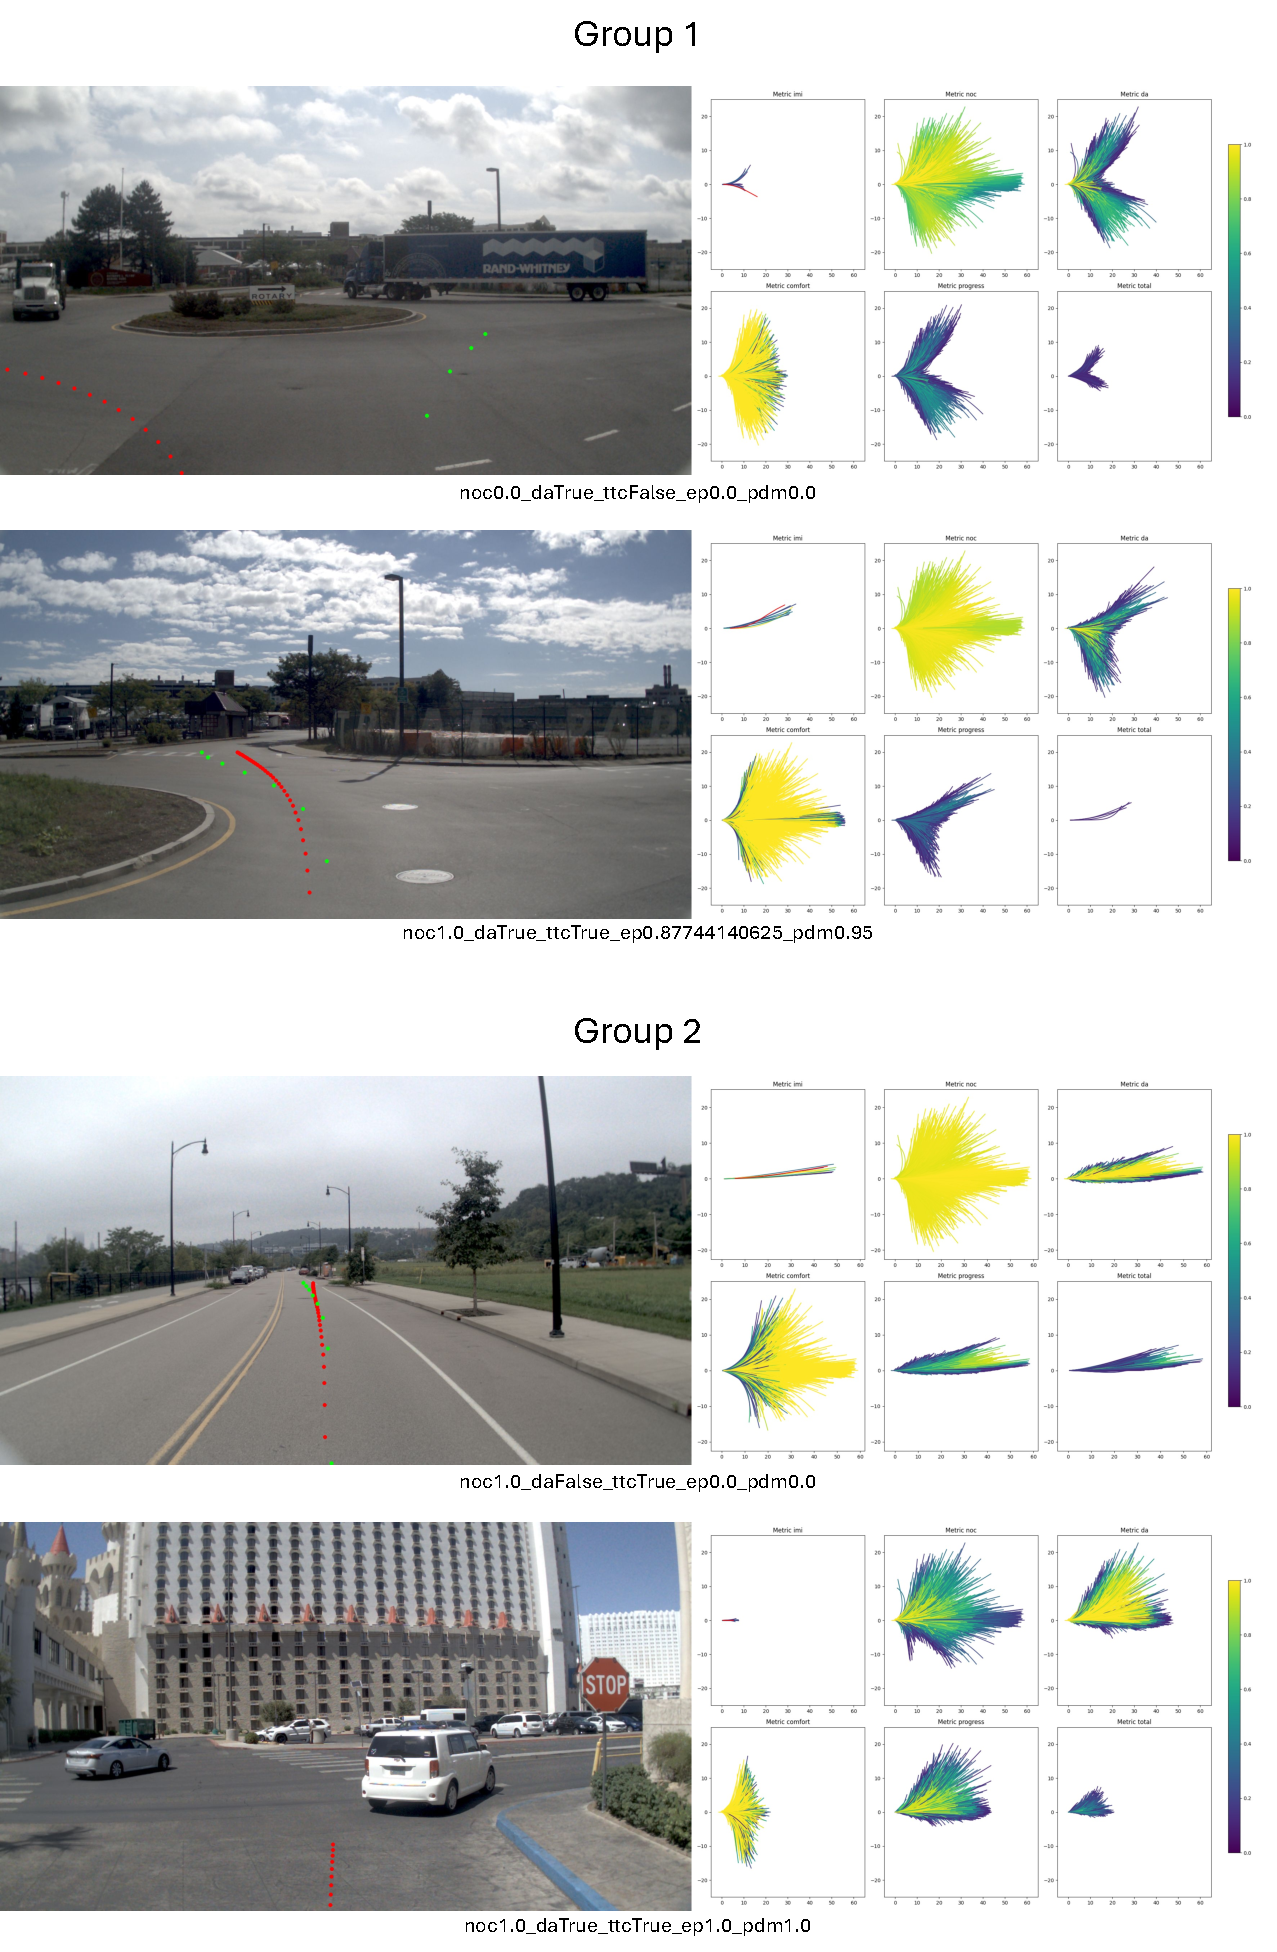
\includegraphics[width=0.55\textwidth]{ch-centaur/images/group12.pdf}
  \caption[Score distributions in success and failure cases]{\textbf{Score distribution differences between success and failure cases.} We show 2 groups of comparisons, with similar scenario types within each group. We observe larger diversity in the failure cases (upper row in each group) than in the successes.}
  \label{centaur:fig:vis_group}
\end{figure}

\subsection{Additional Ablation Studies}\label{centaur:app:ablations}

\begin{table}[t]
  \centering
  \caption[NAVSIM v1.0 comparison to the state of the art]{\textbf{NAVSIM v1.0 comparison to the state of the art.} Unlike the official leaderboard in Table~\ref{centaur:tab:navtest_all}, here we report results for models with a single training seed on the earlier NAVSIM version used for the 2024 NAVSIM Challenge. TransFuser-SE denotes equipping TransFuser with TTT and Semantic Entropy.}
  \label{centaur:tab:navtest_all_supp}
  \begin{adjustbox}{max width=\textwidth}
  \begin{tabular}{ll|cccc|cc}
    \toprule
    \textbf{Model} & \textbf{Deployment} & \textbf{NC} $\uparrow$ & \textbf{DAC} $\uparrow$ & \textbf{EP} $\uparrow$ & \textbf{C} $\uparrow$ & \textbf{TTC} $\uparrow$ & \textbf{PDMS} $\uparrow$ \\
    \midrule
    \multirow{2}{*}{UniAD~\cite{hu2023uniad}} & None & $97.8$ & $91.9$ & $78.8$ & $100.0$ & $92.9$ & $83.4$ \\
    & Optimization & $95.4$ & $86.0$ & $71.9$ & $99.3$ & $87.3$ & $75.2$ \\
    \midrule
    PARA-Drive~\cite{weng2024paradrive} & None & $97.9$ & $92.4$ & $79.3$ & $99.8$ & $93.0$ & $84.0$ \\
    + Occupancy Head & None & $97.8$ & $92.0$ & $78.3$ & $99.7$ & $93.7$ & $83.6$ \\
    \midrule
    TransFuser~\cite{chitta2023transfuser} & None & $97.1$ & $91.9$ & $79.3$ & $100.0$ & $91.9$ & $83.4$ \\
    TransFuser-SE & TTT & $97.9$ & $92.9$ & $80.1$ & $100.0$ & $94.1$ & $85.7$ \\
    \midrule
    DiffusionDrive~\cite{liao2025diffusiondrive} & None & $98.2$ & $96.2$ & $82.2$ & $100.0$ & $94.7$ & $88.1$ \\
    \midrule
    Hydra-MDP~\cite{li2024hydramdp} & None & $98.4$ & $97.8$ & $86.5$ & $100.0$ & $93.9$ & $90.3$ \\
    Hydra-SE & TTT & $99.2$ & $98.5$ & $85.7$ & $100.0$ & $97.1$ & $91.8$ \\
    Centaur & TTT & $99.5$ & $98.9$ & $85.9$ & $100.0$ & $98.0$ & $92.6$ \\
    \bottomrule
  \end{tabular}
  \end{adjustbox}
\end{table}

\paragraph{NAVSIM v1.0.} For completeness, Table~\ref{centaur:tab:navtest_all_supp} compares Centaur with additional baselines on NAVSIM v1.0; in this single-seed comparison, Centaur obtains the highest PDMS of all methods. The table also includes TransFuser-SE, our baseline for applying TTT to trajectory regression models. Similar to Centaur, it obtains an improvement of 2.3 PDMS over its base model, TransFuser without TTT. Interestingly, UniAD~\cite{hu2023uniad}, which uses optimisation with an expert-designed cost function, deteriorates with this optimisation step. This is due to a reduction in ego progress (EP), much like the findings with a fallback layer in Table~\ref{centaur:tab:navtest_ablation}. Furthermore, the results of PARA-Drive~\cite{weng2024paradrive} show that incorporating an explicit representation of 3D occupancy into the end-to-end model can reduce its planning performance. These results show the need for an alternative means of ensuring safety during deployment, such as the proposed TTT.

\begin{table}[t]
  \centering
  \caption[Additional ablations on \texttt{navtest}, with latency]{\textbf{Ablations on \texttt{navtest}.} Additional results complementing Table~\ref{centaur:tab:navtest_ablation}. TTT$^{*}$ combines the history gradients using their SVD instead of averaging them. Hydra-SE$^{\mathbf{f}}$ refers to using $f$ history frames. The shaded row (\colorbox{gray!50}{Hydra-SE$^{\mathbf{4}}$}) applies TTT at inference only on selected frames whose uncertainty is higher than a threshold. We report the \textbf{amortised latency} on \texttt{navtest}.}
  \label{centaur:tab:navtest_ablation_supp}
  \begin{adjustbox}{max width=\textwidth}
  \begin{tabular}{l|ll|rrrr|rr|c}
    \toprule
    \textbf{Model} & \textbf{Deployment} & \textbf{Uncertainty} & \textbf{NC} $\uparrow$ & \textbf{DAC} $\uparrow$ & \textbf{EP} $\uparrow$ & \textbf{C} $\uparrow$ & \textbf{TTC} $\uparrow$ & \textbf{PDMS} $\uparrow$ & \textbf{Latency (ms)} $\downarrow$ \\
    \midrule
    \multirow{4}{*}{TransFuser~\cite{chitta2023transfuser}} & - & - & $97.1$ & $91.9$ & $79.3$ & $100.0$ & $91.9$ & $83.4$ & $103.1$ \\
    & Fallback Layer & Evidential & $98.8$ & $97.4$ & $13.1$ & $100.0$ & $97.9$ & $60.6$ & $108.7$ \\
    & Fallback Layer & Semantic Entropy & $99.2$ & $97.2$ & $14.6$ & $99.8$ & $96.5$ & $59.9$ & $109.9$ \\
    & TTT & Evidential & $97.9$ & $92.5$ & $79.6$ & $100.0$ & $92.9$ & $84.2$ & $149.3$ \\
    \midrule
    \multirow{2}{*}{TransFuser-SE} & TTT & \multirow{2}{*}{Semantic Entropy} & $97.9$ & $92.9$ & $80.1$ & $100.0$ & $94.1$ & $85.7$ & $153.8$ \\
    & TTT$^{*}$ & & $97.4$ & $89.3$ & $78.3$ & $100.0$ & $91.1$ & $83.8$ & $157.6$ \\
    \midrule
    \multirow{4}{*}{Hydra-MDP~\cite{li2024hydramdp}} & - & - & $98.4$ & $97.8$ & $86.5$ & $100.0$ & $93.9$ & $90.3$ & $243.9$ \\
    & Fallback Layer & KL Divergence & $99.1$ & $99.2$ & $9.6$ & $100.0$ & $96.7$ & $63.1$ & $263.2$ \\
    & Fallback Layer & Semantic Entropy & $99.7$ & $99.5$ & $10.4$ & $100.0$ & $98.9$ & $65.3$ & $256.4$ \\
    & TTT & KL Divergence & $98.9$ & $98.1$ & $86.0$ & $100.0$ & $94.4$ & $91.5$ & $357.1$ \\
    \midrule
    \multirow{4}{*}{Hydra-MDP-ViT-L} & - & - & $98.4$ & $97.7$ & $85.0$ & $100.0$ & $94.5$ & $89.9$ & $237.2$ \\
    & Fallback Layer & KL Divergence & $99.7$ & $99.2$ & $10.4$ & $100.0$ & $98.9$ & $67.4$ & $259.5$ \\
    & Fallback Layer & Semantic Entropy & $99.6$ & $97.5$ & $11.8$ & $100.0$ & $94.1$ & $61.0$ & $255.7$ \\
    & TTT & KL Divergence & $99.1$ & $98.2$ & $89.6$ & $100.0$ & $96.7$ & $90.9$ & $354.1$ \\
    \midrule
    Hydra-SE$^{\mathbf{4}}$ & \multirow{4}{*}{TTT} & \multirow{4}{*}{Semantic Entropy} & $99.2$ & $98.5$ & $85.7$ & $100.0$ & $97.1$ & $91.8$ & \multirow{4}{*}{$312.5$} \\
    Hydra-SE$^{\mathbf{3}}$ & & & $98.9$ & $98.7$ & $86.7$ & $100.0$ & $95.1$ & $91.5$ & \\
    Hydra-SE$^{\mathbf{2}}$ & & & $98.8$ & $98.6$ & $86.5$ & $100.0$ & $95.0$ & $91.3$ & \\
    Hydra-SE$^{\mathbf{1}}$ & & & $98.9$ & $98.6$ & $86.7$ & $100.0$ & $95.1$ & $91.4$ & \\
    \midrule
    \rowcolor{gray!50} Hydra-SE$^{\mathbf{4}}$ & TTT & Semantic Entropy & $98.6$ & $98.1$ & $86.3$ & $100.0$ & $94.9$ & $91.3$ & $279.6$ \\
    \bottomrule
  \end{tabular}
  \end{adjustbox}
\end{table}

\begin{table}[t]
  \centering
  \caption[Failure identification with other planners and thresholds]{\textbf{Failure identification.} Additional results complementing Table~\ref{centaur:tab:fail_class}, with other planners and uncertainty thresholds.}
  \label{centaur:tab:fail_class_supp}
  \begin{tabular}{l|l|c|rr}
    \toprule
    \textbf{Uncertainty} & \textbf{Model} & \textbf{Thresh.} & \textbf{TPR} $\uparrow$ & \textbf{Acc.} $\uparrow$ \\
    \midrule
    \multirow{5}{*}{Evidential} & \multirow{5}{*}{TransFuser~\cite{chitta2023transfuser}} & $0.1$ & $47.2$ & $34.9$ \\
    & & $0.3$ & $32.6$ & $48.2$ \\
    & & $0.5$ & $26.9$ & $59.5$ \\
    & & $0.7$ & $23.5$ & $62.8$ \\
    & & $0.9$ & $7.4$ & $71.2$ \\
    \midrule
    KL Divergence & Hydra-MDP~\cite{li2024hydramdp} & $1500$ & $41.3$ & $68.3$ \\
    \midrule
    \multirow{6}{*}{Semantic Entropy} & TransFuser~\cite{chitta2023transfuser} & $0.8$ & $35.3$ & $63.1$ \\
    \cmidrule{2-5}
    & \multirow{5}{*}{Hydra-MDP~\cite{li2024hydramdp}} & $0.2$ & $75.2$ & $61.9$ \\
    & & $0.5$ & $73.3$ & $62.4$ \\
    & & $0.8$ & $62.5$ & $72.2$ \\
    & & $1.1$ & $41.7$ & $73.2$ \\
    & & $1.4$ & $10.9$ & $82.5$ \\
    \midrule
    \textit{Select All} & \multirow{2}{*}{\textit{TransFuser}~\cite{chitta2023transfuser}} & - & $\mathit{100.0}$ & $\mathit{24.1}$ \\
    \textit{Select None} & & - & $\mathit{0.0}$ & $\mathit{75.9}$ \\
    \midrule
    \textit{Select All} & \multirow{2}{*}{\textit{Hydra-MDP}~\cite{li2024hydramdp}} & - & $\mathit{100.0}$ & $\mathit{15.6}$ \\
    \textit{Select None} & & - & $\mathit{0.0}$ & $\mathit{84.4}$ \\
    \bottomrule
  \end{tabular}
\end{table}

\paragraph{Latency.} We count the forward pass time in milliseconds. For planners with uncertainty estimation and a deployment strategy, we count the forward pass time once and then add the time for the corresponding deployment method (test-time training or fallback layer). For test-time training, we include the time for the gradient calculation as well as the model update; for the fallback layer, we include the nearest-neighbour search that selects the safe trajectory closest to the predicted trajectory in terms of $L_2$ distance. The hardware used for this inference test is as follows:
\begin{itemize}
  \item GPU: 1 $\times$ NVIDIA A100, driver version 535.54.03;
  \item CPU: AMD EPYC 9124 16-Core Processor;
  \item RAM: 500\,GB.
\end{itemize}
As shown in Table~\ref{centaur:tab:navtest_ablation_supp}, a direct comparison of the base TransFuser and Hydra-MDP models, without the proposed deployment and uncertainty enhancements, reveals a significant performance gap in favour of Hydra-MDP. This can be attributed to their different backbone architectures. TransFuser uses an efficient ResNet-34 backbone which, although it sacrifices performance, has a substantially lower latency of 103.1\,ms, compared with 243.9\,ms for Hydra-MDP. In contrast, the more computationally expensive \mbox{V2-99} backbone of Hydra-MDP contributes to its higher performance by around 7 PDMS. We reiterate that the gradient calculation time is currently included in the latency measured for TTT methods. It could be reduced by parallelising execution in our implementation, or by applying TTT only on selected frames where the uncertainty exceeds a threshold (Table~\ref{centaur:tab:navtest_ablation_supp}, bottom row).

\paragraph{TTT with SVD.} Following~\cite{Gao2024fstta}, an alternative implementation of test-time adaptation applies singular-value decomposition (SVD) to the history gradients to find the most useful ones for updating the model. As shown in Table~\ref{centaur:tab:navtest_ablation_supp}, in our case TTT$^{*}$ (using SVD) performs worse on TransFuser-SE than TTT with averaged gradients.

\paragraph{ViT-L backbone.} Table~\ref{centaur:tab:navtest_ablation_supp} also ablates the influence of different backbones on Hydra-MDP under different uncertainty measures and deployment strategies. Overall, the \mbox{V2-99} backbone used in Hydra-MDP performs better than the ViT-L backbone. However, with a fallback layer and KL Divergence, the ViT-L backbone surpasses \mbox{V2-99} by around 4 PDMS.

\paragraph{Buffer length $F$.} Table~\ref{centaur:tab:navtest_ablation_supp} shows the influence of the number of history frames used by Hydra-SE on \texttt{navtest}. We observe a slight performance gain when increasing the number of history frames ($F=2$ gives the lowest performance). Overall, the performance is consistent across all settings of $F$, indicating the robustness of the approach.

\paragraph{Failure identification thresholds.} Table~\ref{centaur:tab:fail_class_supp} investigates the effect of different uncertainty thresholds on the identification of possible failure cases. For both TransFuser with evidential uncertainty and Hydra-MDP with Semantic Entropy, increasing the threshold decreases the TPR for failure cases and increases the overall accuracy. The reason is that \texttt{navtest} has a long-tailed distribution in which failure cases account for a small portion of the test samples, which makes it hard to pick true failure cases without misidentifying true successes. Consequently, at every threshold listed, the accuracy of each measure stays below that of the corresponding Select None baseline. Threshold-free metrics such as AUROC, which would summarise the whole trade-off between true and false positives, were not reported.
